\subsection{Desarrollo de la aplicación móvil}

\subsubsection{Introducción}
El desarrollo de la aplicación se puede dividir en cuatro fases distintas, la primer fase incluye la comunicación bluetooth con el sensor, la segunda la generación del mapa que se muestra al usuario mediante el uso del API de Google Maps, la tercera se refiere al desarrollo nativo de la aplicación móvil usando el lenguaje de programación Java, finalmente, la cuarta y última fase, consiste en la conexión de la aplicación móvil con el servidor web mediante el uso de la librería para Android ``Retrofit''. Donde la aplicación móvil funcionará como la capa de presentación para el usuario (frontend), mientras que en el servidor web se alojará toda la lógica del negocio así como la base de datos (backend).

\subsubsection{Comunicación Bluetooth}
En lo referente a la comunicación entre el sensor y la aplicación móvil se utilizo el protocolo de comunicación bluetooth, los que se serán recibidos por la aplicación será el valor de la frecuencia en cada segundo, por lo tanto dentro de la aplicación móvil se realiza el calculo de flujo de combustible.
\newline
Para iniciar la comunicación en la aplicación se necesita principalmente de dos métodos realizados en java.El primero se encarga de recibir las solicitud de conexiones entrantes y al aceptar una proporcionar un socket de conexión.
El código se muestra a continuación:
\lstinputlisting[language=Java]{Capitulo5/software/submodulos/aplicacion/src/AcceptThread.java}
A fin de inicializar una conexión con un dispositivo remoto, primero se obtiene un objeto BluetoothDevice que represente el dispositivo remoto y posteriormente, se usa el BluetoothDevice para obtener un BluetoothSocket e inicializar la conexión.
A continuación se muestra el código referente a lo dicho anteriormente.
\lstinputlisting[language=Java]{Capitulo5/software/submodulos/aplicacion/src/ConnectThread.java}

\subsubsection{Generación del mapa}

Para la generación del mapa, se definió que el API con que se trabaría fuera el API de Google Maps, debido a que hoy en día es una herramienta muy poderosa que nos brinda muchas herramientas para trabajar más agílmente. Además, el precio por usar la API es gratuito para los fines que se le dará durante la elaboración del presente proyecto. En caso de escalar y llegar a más usuarios el costo de usar la API variaría dependiendo de la cantidad de peticiones que usemos, en lugar de tener una tarifa fija.\\ Para realizar la integración entre nuestra aplicación y el API de Google Maps, fue necesario, crear una credencial de API desde la Consola de Google APIs (Console Google APIs).\\ A continuación, se detalla el procedimiento que se realizó para poder obtener una credencial para usar el API.\\En la Figura \ref{fig:consola_google}, se muestra el sitio web correspondiente a la consola de Google APIs, el cual después de registrarse usando una cuenta de Google, te muestra información detallada del uso que les has dado a las APIs de Google desde alguna de tus credenciales generadas (en caso de existir). 

\begin{figure}[H]
	\centering
	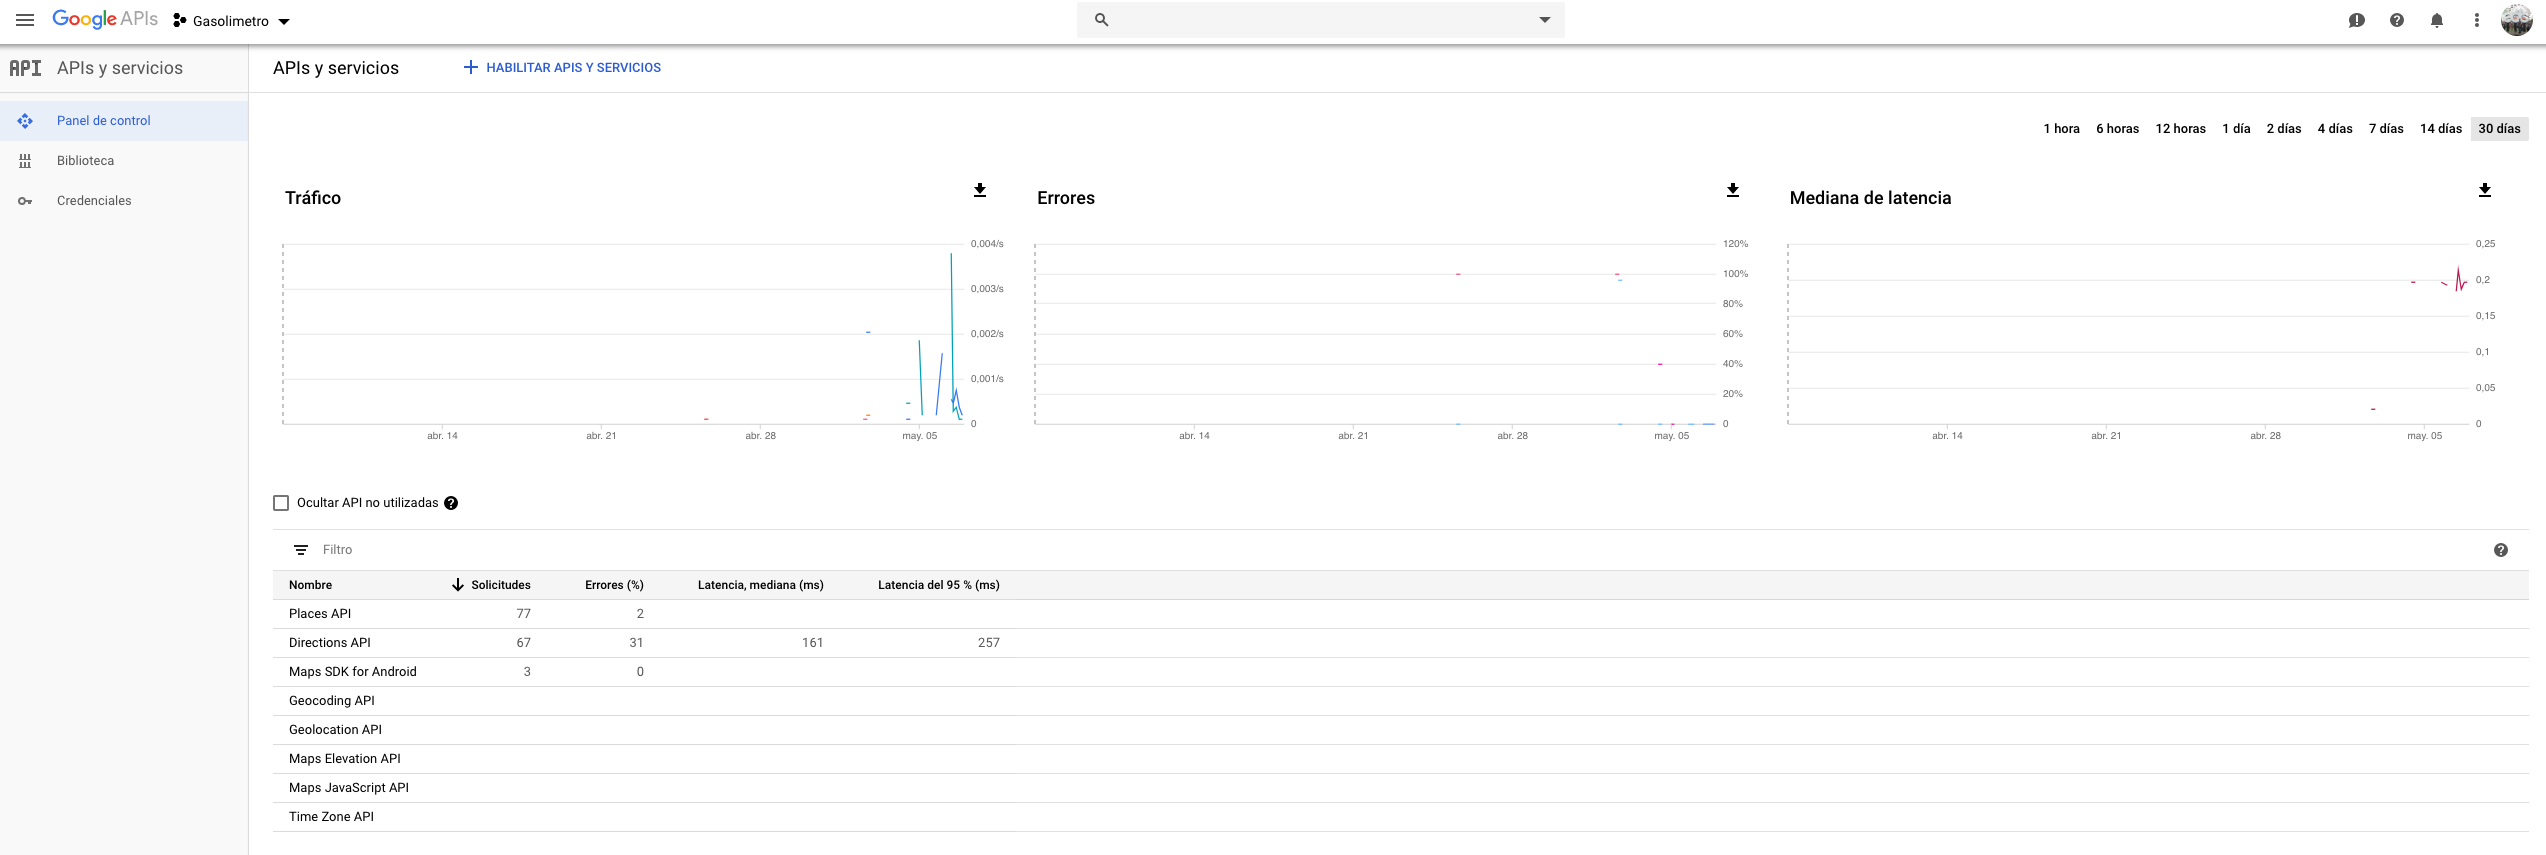
\includegraphics[scale=.18]{Capitulo5/software/submodulos/aplicacion/images/1}
	\caption{Captura de pantalla de la Consola Google APIs}
	\label{fig:consola_google}
\end{figure}

Para poder crear una credencial y posteriormente usarla en nuestra aplicación, ese necesario ``habilitar'', para nuestra cuenta o proyecto, el API que requerimos usar, para ello, debemos dar click, sobre el botón ``HABILITAR APIS Y SERVICIOS'' que se muestra en la parte superior izquierda de la pantalla mostrada en la Figura \ref{fig:consola_google}, el cual nos mostrará una pantalla como la que se muestra en la Figura \ref{fig:consola_google2}, la cual es un menú que indica todas las APIs de Google disponibles, y al seleccionar alguna, se nos mostrará una pantalla como se muestra en la Figura \ref{fig:consola_google3}, con la diferencia de que al hacerlo por primera vez, el API estará deshabilitado.\\En este caso particular, las APIs que se requirieron ``habilitar'' fueron las siguientes:
\begin{itemize}
	\item \textbf{Maps SDK for Android}: Para poder mostrar el mapa desde Android nativo.
	\item \textbf{Directions API}: Para poder trazar rutas desde un punto de inicio a un punto de destino en el mapa.
	\item \textbf{Places API}: Para mostrar información al usuario sobre un punto específico en el mapa, puntualmente se obtienen solamente latitud, longitud y la dirección del mismo.
\end{itemize}

\begin{figure}[H]
	\centering
	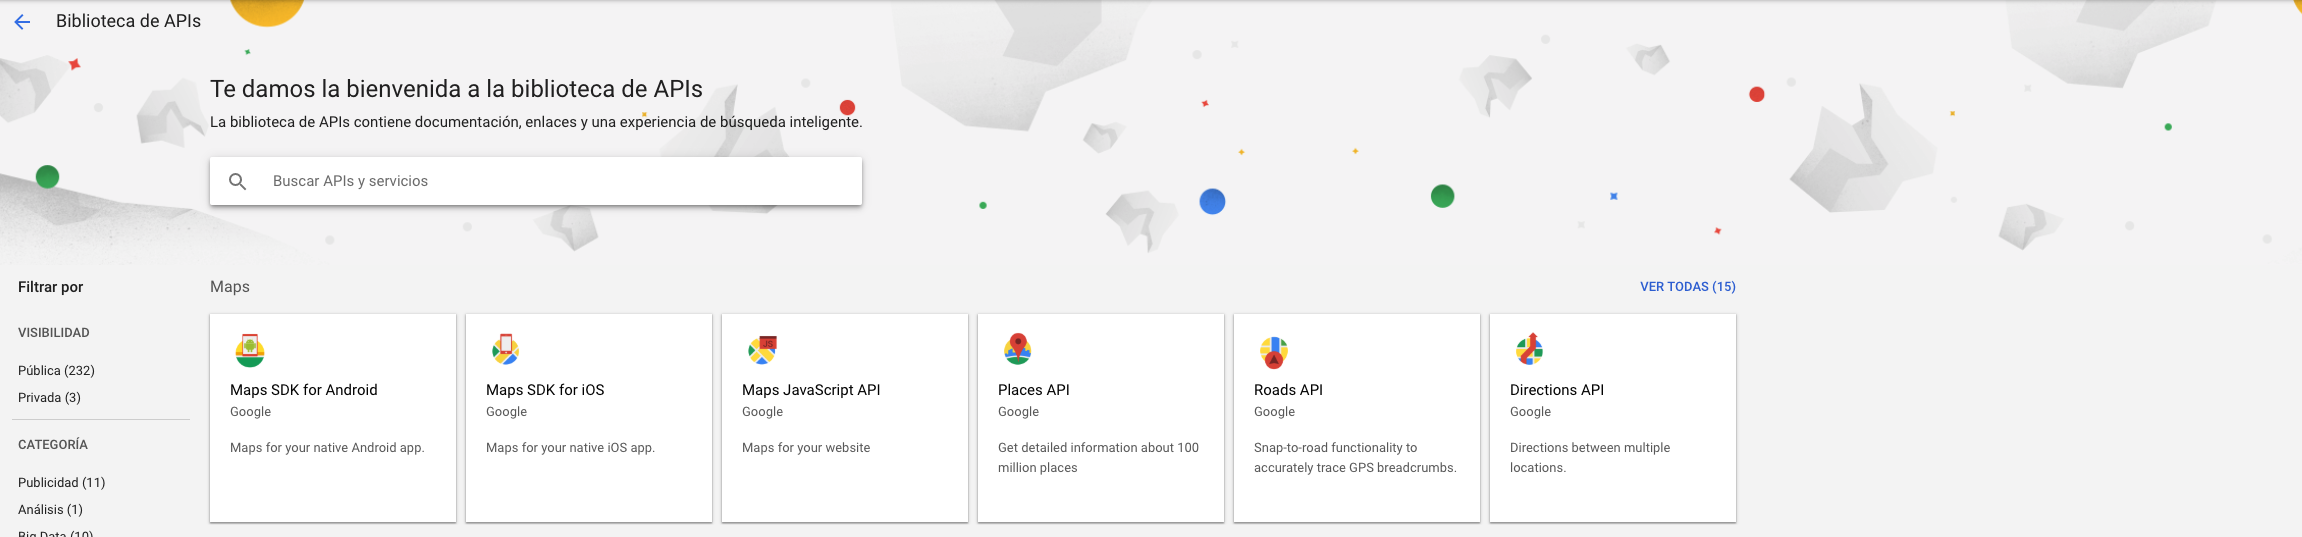
\includegraphics[scale=.2]{Capitulo5/software/submodulos/aplicacion/images/2}
	\caption{Captura de pantalla del menú de APIs de Google}
	\label{fig:consola_google2}
\end{figure}

Las Figuras \ref{fig:consola_google3}, \ref{fig:consola_google4} y \ref{fig:consola_google5} muestran como están habilitadas cada una de las APIs descritas anteriormente.

\begin{figure}[H]
	\centering
	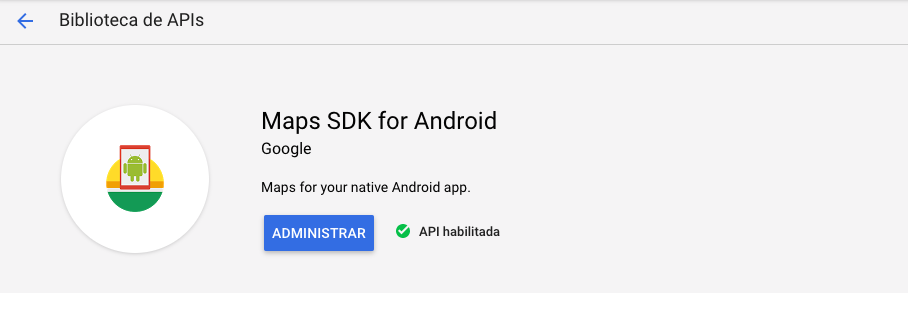
\includegraphics[scale=.3]{Capitulo5/software/submodulos/aplicacion/images/3}
	\caption{Captura de pantalla del SDK de Android habilitado}
	\label{fig:consola_google3}
\end{figure}

\begin{figure}[H]
	\centering
	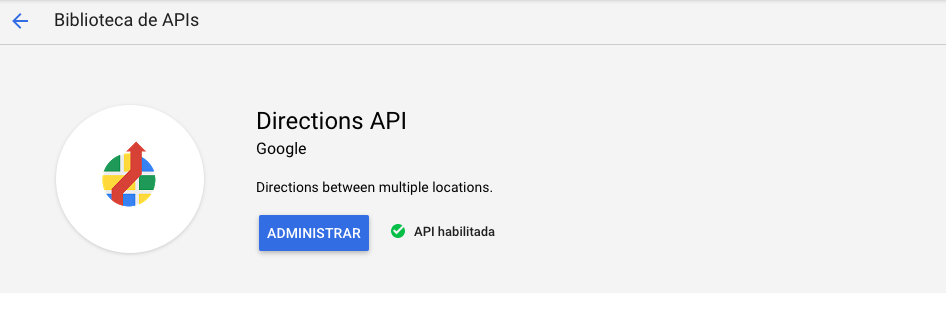
\includegraphics[scale=.3]{Capitulo5/software/submodulos/aplicacion/images/4}
	\caption{Captura de pantalla del API de Directions habilitado}
	\label{fig:consola_google4}
\end{figure}

\begin{figure}[H]
	\centering
	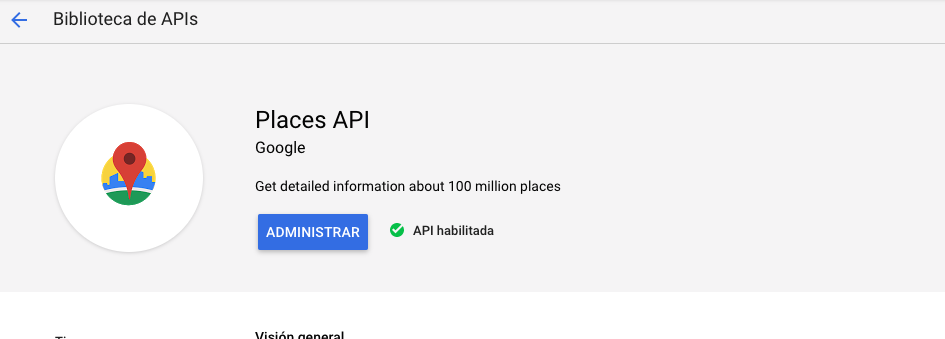
\includegraphics[scale=.3]{Capitulo5/software/submodulos/aplicacion/images/5}
	\caption{Captura de pantalla del API de Places habilitado}
	\label{fig:consola_google5}
\end{figure}

Finalmente, cuando se habilita cualquier de las APIs posteriores, Google generará automáticamente una credencial de API con el que se pueda trabajar, es posible editar información de está API y limitar su uso para solo ciertos dispositivos, como se muestra la Figura \ref{fig:consola_google6}.

\begin{figure}[H]
	\centering
	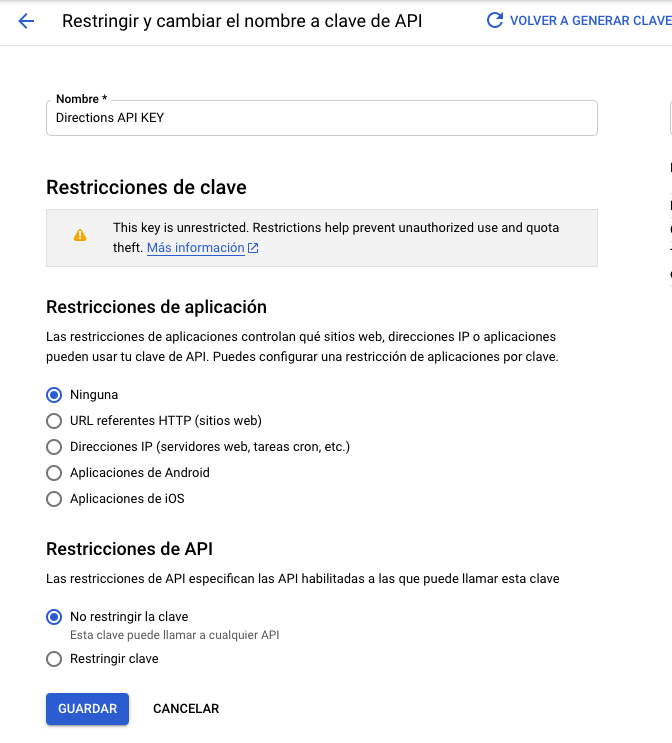
\includegraphics[scale=.4]{Capitulo5/software/submodulos/aplicacion/images/6}
	\caption{Captura de pantalla de credencial generada}
	\label{fig:consola_google6}
\end{figure}

Para el presente proyecto, se usan dos credenciales distintas, una para las peticiones hacía el ``Maps SDK for Android'' y otra para las consultar hacía ``Directions API'' y ``Places API''.\\

Posteriormente a tener las credenciales necesarias, sigue el paso de comunicarse con las distintas APIs y trabajar con sus respuestas. En el caso del SDK, dado que es especial para el uso con Android, no es necesario dar un tratamiento particular a las respuestas de este, ya que todo se encuentra definido en código Java como clases. Sin embargo, tanto Directions como Places, cuando son consultadas, nos devuelven información en formato ``JSON'' de la forma clave-valor. Es por ello que resulta necesario tener un trabajo previo de procesamiento de la respuesta antes de poder trabajar con los datos de forma nativa en Android.\\

En el siguiente fragmento de código, muestra una respuesta json de la API de Directions.\\

json-lugares.json
\lstinputlisting[language=Java]{Capitulo5/software/submodulos/aplicacion/src/json-places.json}

En el siguiente fragmento de código, muestra una respuesta json de la API de Places.\\

json-lugar.json

\lstinputlisting[language=Java]{Capitulo5/software/submodulos/aplicacion/src/json-place.json}

El primer archivo json mostrado, tiene su equivalente en Java como se muestra a continuación.\\

Lugares.java

\lstinputlisting[language=Java]{Capitulo5/software/submodulos/aplicacion/src/PlaceFeed.java}

Para el segundo archivo json, que corresponde a la información de un solo lugar, su equivalente en Java es el siguiente.\\

Lugar.java

\lstinputlisting[language=Java]{Capitulo5/software/submodulos/aplicacion/src/ResultPlace.java}

A su vez, las clases Java mostradas anteriormente, hacen uso de otras clases Java para definir algunas de sus propiedades, las más importantes para el presente trabajo, son aquellas que contienen la información geográfica del lugar (latitud y longitud). Estas clases son Geometria y Ubicacion respectivamente.\\

Geometria.java

\lstinputlisting[language=Java]{Capitulo5/software/submodulos/aplicacion/src/Geometry.java}

Ubicacion.java
\lstinputlisting[language=Java]{Capitulo5/software/submodulos/aplicacion/src/Location.java}

Finalmente, todo lo anterior puede verse reflejado en la implementación de una función que obtenga información para mostrar en el mapa, como la función ``inicializarUbicacion()'' del archivo ConsultarMapa.java.\\

inicializarUbicacion() del archivo ConsultarMapa.java 

\lstinputlisting[language=Java]{Capitulo5/software/submodulos/aplicacion/src/initLocation.java}

\subsubsection{Desarrollo de la app móvil}

Para el desarrollo del resto de la aplicación, la gran mayoría de funcionalidades corresponden a ``CRUDS'' (altas, bajas, cambios y consultas por sus siglas en inglés), por lo cual no resulta de interés explica más a fondo su implementación, sin embargo, resulta necesario explicar en este apartado, como es que se trabajo con el bluetooth en el dispositivo Android, debido a que esto es más complejo.\\

Primero, es necesario especificar en nuestro archivo ``AndroidManifest.xml'' del proyecto, todos los permisos necesarios para poder obtener acceso a la red del dispositivo móvil (Internet), a la posición mediante el GPS, y al conector Bluetooth del mismo. Estos permisos deben ser definidos de la siguiente manera:\\AndroidManifest.xml

\lstinputlisting[language=XML]{Capitulo5/software/submodulos/aplicacion/src/manifest.xml}

Finalmente, para trabajar con el conector Bluetooth del dispositivo móvil, es necesario realizar diversas validaciones, como por ejemplo, que el dispositivo móvil lo tenga, que este activado, y que la aplicación tenga permiso de usarlo. A continuación se muestra un fragmento de código que verifica que el dispositivo móvil tenga Bluetooth.\\

verificarBluetooth() de ConsultarMapaMenu.java

\lstinputlisting[language=Java]{Capitulo5/software/submodulos/aplicacion/src/bluetooth.java}

\subsubsection{Comunicación con el servidor web}

Para la comunicación con nuestro propio servidor web, y las APIs de Google, se uso la librería ``Retrofit'' en su versión 2 (Retrofit2). Ya que nos provee de clases e interfaces en Java, las cuales permiten trabajar de forma más sencilla la comunicación con servidores mediante el uso del protocolo HTTP.\\ Para trabajar con está librería, en primer instancia en necesario agregarla a nuestro archivo de configuración de la aplicación de gradle. Posteriormente es necesario crear una interfaz que contenga un método por cada URL a la que nos esteremos conectando, a continuación, se muestra el archivo ``RestClient,java'', el cual es nuestra interfaz definida para el proyecto.\\Restclient.java

\lstinputlisting[language=Java]{Capitulo5/software/submodulos/aplicacion/src/RestClient.java}

Opcionalmente, también se puede crear un archivo con funciones útiles para trabajar con Retrofit, el archivo que se muestra a continuación, corresponde a nuestro archivo de utilerias del proyecto. Solo contiene una función la cual nos permite crear una nueva instancia de la clase ``Retrofit''.\\RetrofitUtils.java
\lstinputlisting[language=Java]{Capitulo5/software/submodulos/aplicacion/src/RetrofitUtils.java}

Finalmente, al unir lo anterior, podemos definir funciones que se comuniquen con un servidor web para obtener información que pueda ser procesada posteriormente. El siguiente fragmento de código corresponde a la función ``obtenerGasolinerasCercanasGoogle()'' del archivo ``ConsultarMapa.javaa'', en esta función, se obtienen las gasolineras cercanas a la posición actual del usuario, puntualmente en un radio definido como regla de negocio.
\\obtenerGasolinerasCercanasGoogle() de ConsultarMapa.java
\lstinputlisting[language=Java]{Capitulo5/software/submodulos/aplicacion/src/obtenerGasolineras.java}


